\documentclass[spanish, 10pt,a4paper]{article}
\usepackage[spanish]{babel}
\usepackage[utf8]{inputenc}
\usepackage{textcomp}
\usepackage{hyperref}
\usepackage[pdftex]{graphicx}
\usepackage{epsfig}
\usepackage{amsmath}
\usepackage{hyperref}
\usepackage{amssymb}
\usepackage{color}
\usepackage{graphics}
\usepackage{amsthm}
\usepackage{subcaption}
\usepackage{caratula}
\usepackage{fancyhdr,lastpage}
\usepackage[paper=a4paper, left=1.4cm, right=1.4cm, bottom=1.4cm, top=1.4cm]{geometry}
\usepackage[table]{xcolor} % color en las matrices
\usepackage[font=small,labelfont=bf]{caption} % caption de las figuras en letra mas chica que el texto
\usepackage{listings}
\usepackage{float}
\usepackage{pdfpages}
\usepackage{amsfonts}
\usepackage{upgreek}


\color{black}

%%%PAGE LAYOUT%%%
\topmargin = -1.2cm
\voffset = 0cm
\hoffset = 0em
\textwidth = 48em
\textheight = 164 ex
\oddsidemargin = 0.5 em
\parindent = 2 em
\parskip = 3 pt
\footskip = 7ex
\headheight = 20pt
\pagestyle{fancy}
\lhead{IS1 - Trabajo Pr\'actico 1} % cambia la parte izquierda del encabezado
\renewcommand{\sectionmark}[1]{\markboth{#1}{}} % cambia la parte derecha del encabezado
\rfoot{\thepage}
\cfoot{}
\numberwithin{equation}{section} %sets equation numbers <chapter>.<section>.<subsection>.<index>

\newcommand{\figurewidth}{1\textwidth}

\newcommand{\tuple}[1]{\ensuremath{\left \langle #1 \right \rangle }}
\newcommand{\Ode}[1]{\small{$\mathcal{O}(#1)$}}


%El siguiente paquete permite escribir la caratula facilmente
\hypersetup{
  pdftitle={ IS1 - TP1 },
  colorlinks,
  citecolor=black,
  filecolor=black,
  linkcolor=black,
  urlcolor=black 
}

\materia{Ingeniería de Software I}

\titulo{Trabajo Práctico 1}

\subtitulo{Informe y diagramas.}

\grupo{Grupo 2}

\integrante{De Sousa Bispo, Germán}{359/12}{germandesousa@gmail.com}
\integrante{Fernandez, Esteban}{691/12}{esteban.pmf@gmail.com}
\integrante{Kodelia, Erika Natasha}{767/11}{erikankodelia@gmail.com}
\integrante{Mongi Badia, Martín}{422/13}{martinmongi@gmail.com}
\integrante{Sánchez Cano, Gonzalo}{}{xeneize__86@hotmail.com}
\integrante{Wright, Carolina}{876/12}{wright.carolina@gmail.com}

 
\begin{document}
{ \oddsidemargin = 2em
	\headheight = -20pt
	\maketitle
}
	\tableofcontents
	\newpage
\section{Introducción}
	El Ministro de Gobierno quiere modificar el Sistema Electoral Nacional y para ello propone instalar en las escuelas máquinas emisoras de sufragios. Junto con esta incorporación se deberá modificar el Sistema del Centro de Cómputos Nacional para que pueda operar con las máquinas.

	El formato de la votación no presenta cambios, es decir, al igual que en el sistema de boletas que se venía utilizando se permitirá votar por categorías o votar en blanco. 
	
	Además se busca proveer todos los mecanimos necesarios para asegurar el derecho de voto a todos los Electores. Se considerarán las necesidades de los no videntes y personas con movilidad reducida. 
	
\section{Presunciones}

\section{Vistas}
	A continuación se visualizarán los diagramas realizados junto con la explicación necesaria para cada tipo:
\subsection{Diagrama de Contexto}
	Se agrega el diagrama de contexto entregado en el trabajo práctico anterior con las modificaciones necesarias para adptarse a los O-refinamientos elegidos. Esto corresponde a no realizar una autenticación por parte del Elector a la máquina de sufragio a la hora de realizar la votación (alcanza con insertar la boleta). Además, la habilitación del modo audio de la máquina de sufragio por parte del Presidente de Mesa se realiza solamente a través de la inserción de los auriculares. 
\par El diagrama de contexto resultante es el siguiente:

\vspace{\baselineskip}
    \begin{center}
                \includegraphics[scale=0.40]{imagenes/contexto/DiagramaDeContextoTP2.png}
                \\
                \vspace{1pt}
                \footnotesize\textit{}
        \end{center}
\vspace{\baselineskip}


\subsection{Diagrama de Caso de Uso}

\vspace{\baselineskip}
    \begin{center}
                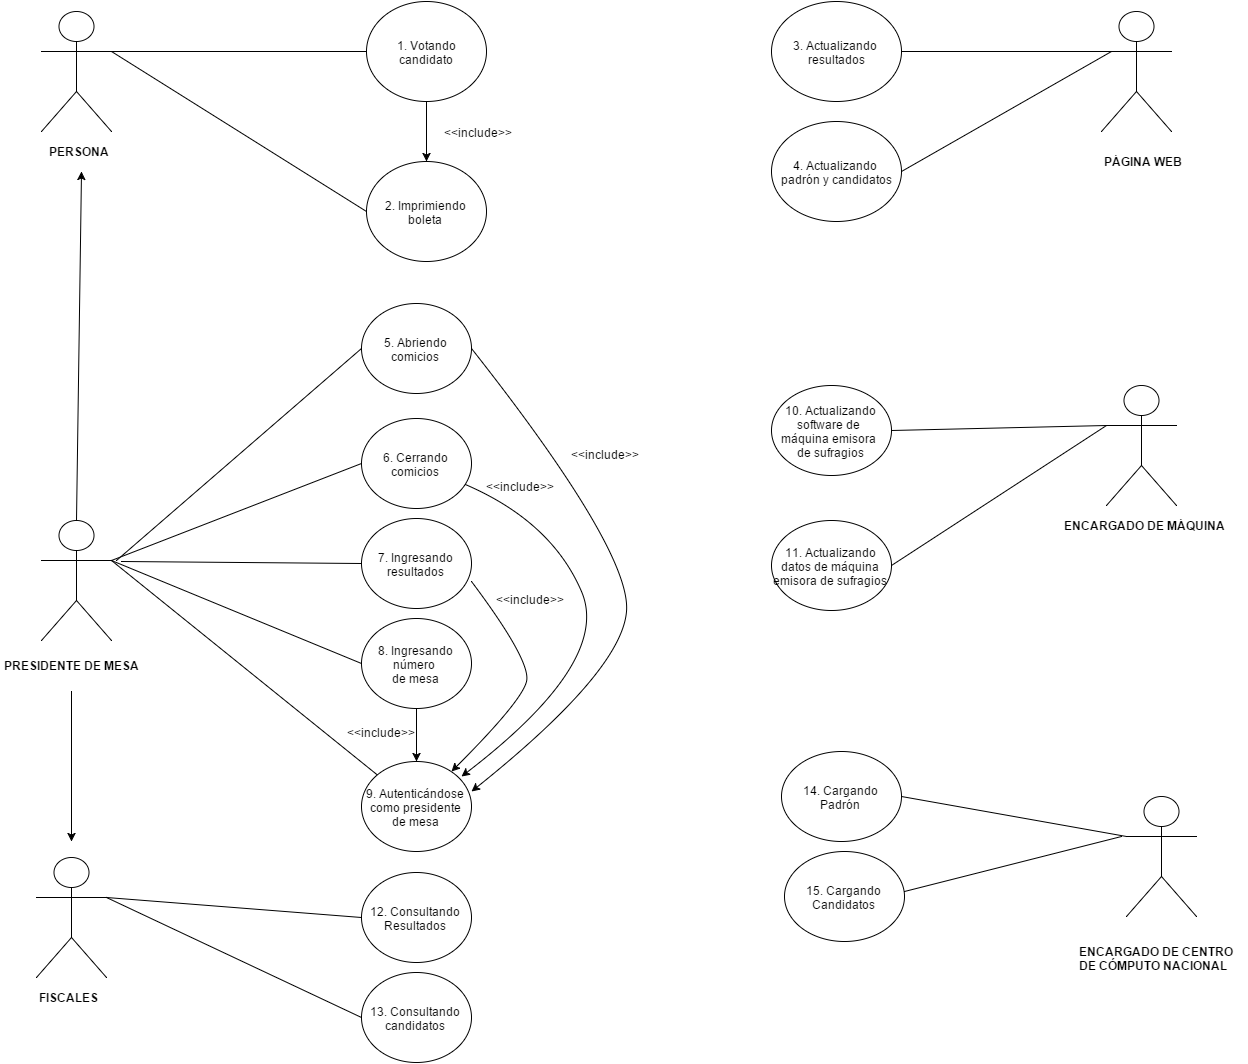
\includegraphics[scale=0.40]{imagenes/CasosDeUso.png}
                \\
                \vspace{1pt}
                \footnotesize\textit{}
        \end{center}
\vspace{\baselineskip}

\newpage

\noindent\textbf{Detalle de Casos de Uso:}\\

\noindent\textbf{Caso de Uso: Votando candidatos}\\
\textbf{Actor: } Persona.\\
\textbf{Pre: } Se abrieron los comicios.\\
\textbf{Post: } La persona logra registrar su voto.\\
\begin{table}[H]
  \centering
\bgroup
\def\arraystretch{1.3}
  \begin{tabular}{p{9cm} | p{7cm}}
    \hline
    Curso Normal & Curso Alternativo \\
    \hline
    \hline    
    1. La \textbf{\textit{persona}} ingresa la \textit{boleta de votación}. 
    & \\
    
    \hline
    2. El \textbf{\textit{SVE}} brinda toda la información en este CU, tanto por pantalla como por audio a través de una salida por auricular.
    &
    \\
    
    \hline
    3 El \textbf{\textit{SVE}} verifica que sea una \textit{boleta de votación}.
    & 
    3.1 En el caso que no sea una boleta válida, el \textbf{\textit{SVE}} entrega el mensaje de \textit{''Error de boleta''}
    \\
    
    \hline
    4 El \textbf{\textit{SVE}} le brinda a la persona, las opciones de \textit{''votar lista completa''} y \textit{''votar por categorías''}.
    & 
    4.1 En el caso en que no se pueda mostrar la información necesaria, el \textbf{\textit{SVE}} entrega el mensaje de \textit{''Error de interfaz''}
    \\
    
    \hline
    5 La \textbf{\textit{persona}} elije una de las dos opciones mostradas en el paso anterior.
    & \\
    
    \hline
    6 Si la \textbf{\textit{persona}} eligió lista completa, continúo con el \textbf{\textit{paso 14}}.
    & \\
    
    \hline
    7 El \textbf{\textit{SVE}} muestra como opciones distintas a cada uno de los candidatos de una categoría y otra opción de \textit{''votar en blanco''}.
    & 
    7.1 En el caso en que no se pueda mostrar la información necesaria, el \textbf{\textit{SVE}} entrega el mensaje de \textit{''Error de interfaz''}
    \\
    
    \hline
    8 La \textbf{\textit{persona}} elije una de las opciones mostradas en el paso anterior.
    & \\
    
    \hline
    9 El \textbf{\textit{SVE}} verifica que se hayan votado todas las categorías. Si falta votar alguna categoría, continúo con la siguiente categoría y sigo con el \textbf{\textit{paso 7}}.
    & \\
    
    \hline
    10 El \textbf{\textit{SVE}} mostrará la elección de cada uno de los candidatos elegidos por la persona, para que la misma pueda verificarlos.
    & \\
    
    \hline
    11 La \textbf{\textit{persona}} confirmará que desea realizar esa votación.
    & 
    11.1 En el caso en que la \textbf{\textit{persona}} no desee confirmar la votación y haya elegido realizarla nuevamente, voy al \textbf{\textit{paso 3}}.\\
    
    \hline
    12 El \textbf{\textit{SVE}} registra el voto.
    & 
    12.1 En el caso en que no se pueda registrar el voto, el \textbf{\textit{SVE}} entrega el mensaje de \textit{''Error de registración''}
    \\
    
    \hline
    13 Fin de CU
    & \\
    
    \hline
    14 El \textbf{\textit{SVE}} muestra como opciones distintas a cada uno de las listas completas de los candidatos y otra opción de \textit{''votar en blanco''}.
    & 
    14.1 En el caso en que no se pueda mostrar la información necesaria, el \textbf{\textit{SVE}} entrega el mensaje de \textit{''Error de interfaz''}
    \\
    
    \hline
    15 La \textbf{\textit{persona}} elije una de las opciones mostradas en el paso anterior, y continúo en el \textbf{\textit{paso 10}}.
    & \\
    \hline
  \end{tabular}
\egroup
\end{table}


\newpage
\noindent\textbf{Caso de Uso: Imprimiendo boleta}\\
\textbf{Actor: } Persona.\\
\textbf{Pre: } Se confirmó el voto y se encuentra ingresada la boleta de votación.\\
\textbf{Post: } Se imprime la boleta.\\
\begin{table}[H]
  \centering
\bgroup
\def\arraystretch{1.3}
  \begin{tabular}{p{9cm} | p{7cm}}
    \hline
    Curso Normal & Curso Alternativo \\
    \hline
    \hline    
    1. La \textbf{\textit{persona}} selecciona la opción de \textit{''Imprimir boleta''}. 
    & \\
    
    \hline
    2. El \textbf{\textit{SVE}} imprime la boleta.
    &
    2.1 En el caso en que no se pueda imprimir la boleta, el \textbf{\textit{SVE}} entrega el mensaje de \textit{''Error de impresión''}
    \\
    
    \hline
    3 Fin de CU
    & \\
    \hline
  \end{tabular}
\egroup
\end{table}


\noindent\textbf{Caso de Uso: Actualizando información de página web}\\
\textbf{Actor: } Página web.\\
\textbf{Pre: } Se cerraron los comicios.\\
\textbf{Post: } Se actualiza la información de los resultados en la página web.\\
\begin{table}[H]
  \centering
  \begin{tabular}{p{9cm} | p{7cm}}
    \hline
    Curso Normal & Curso Alternativo \\
    \hline
    \hline    
    1. La \textbf{\textit{Página web}} consulta resultados al \textbf{\textit{SVE}}. 
    & \\
    
    \hline
    2. El \textbf{\textit{SVE}} brinda satisfactoriamente la información a la página web
    & 
    2.1 Si el \textbf{\textit{SVE}} no puede brindar la información, se mostrará un mensaje de \textit{''Error de actualización de resultados''} en la página web.
    \\
    
    \hline
    3. La \textbf{\textit{Página web}} actualizará los resultados en la página web.
    & \\
    \hline
  \end{tabular}
\end{table}


\noindent\textbf{Caso de Uso: Actualizando padrón y candidatos}\\
\textbf{Actor: } Página web.\\
\textbf{Pre: } Faltan por lo menos 24hs para la apertura de los comicios.\\
\textbf{Post: } Se actualiza la información del padrón y de los candidatos en la página web.\\
\begin{table}[H]
  \centering
  \begin{tabular}{p{9cm} | p{7cm}}
    \hline
    Curso Normal & Curso Alternativo \\
    \hline
    \hline    
    1. La \textbf{\textit{Página web}} consulta el padrón y los candidatos al \textbf{\textit{SVE}}. 
    & \\
    
    \hline
    2. El \textbf{\textit{SVE}} brinda satisfactoriamente la información a la \textbf{\textit{Página web}}
    & 
    2.1 Si el \textbf{\textit{SVE}} no puede brindar la información, se mostrará un mensaje de \textit{''Error de actualización de padrón y candidatos''} en la página web.
    \\
    
    \hline
    3. La \textbf{\textit{Página web}} actualizará el padrón y los candidatos en la página web.
    & \\
    \hline
  \end{tabular}
\end{table}


\newpage
\noindent\textbf{Caso de Uso: Abriendo comicios}\\
\textbf{Actor: } Presidente de mesa.\\
\textbf{Pre: } Los comicios no se encuentran abiertos.\\
\textbf{Post: } Se abren los comicios.\\
\begin{table}[H]
  \centering
\bgroup
\def\arraystretch{1.3}
  \begin{tabular}{p{9cm} | p{7cm}}
    \hline
    Curso Normal & Curso Alternativo \\
    \hline
    \hline    
    1. El \textbf{\textit{presidente de mesa}} ingresa la \textit{boleta de presidente de mesa}. 
    & \\
    
    \hline
    2. El \textbf{\textit{SVE}} brinda toda la información en este CU, tanto por pantalla como por audio a través de una salida por auricular.
    &
    \\
    
    \hline
    3 El \textbf{\textit{SVE}} verifica que sea una \textit{boleta de presidente de mesa}.
    & 
    3.1 En el caso que no sea una boleta válida, el \textbf{\textit{SVE}} entrega el mensaje de \textit{''Error de boleta''}
    \\
    
    \hline
    4 El \textbf{\textit{SVE}} le brinda a la persona, las opciones de \textit{''abrir comicios''}, \textit{''cerrar comicios''}, \textit{''ingresar resultados''} y \textit{''ingresar número de mesa''}.
    & 
    4.1 En el caso en que no se pueda mostrar la información necesaria, el \textbf{\textit{SVE}} entrega el mensaje de \textit{''Error de interfaz''}
    \\
    
    \hline
    5 El \textbf{\textit{presidente de mesa}} elije la opcion de \textit{''abrir comicios''}.
    & \\
    
    \hline
    6. El \textbf{\textit{SVE}} registra la apertura de los comicios.
    &
    6.1 En el caso en que no se pueda registrar la apertura, el \textbf{\textit{SVE}} entrega el mensaje de \textit{''Error de registración''}
    \\
    
    \hline
    7 Fin de CU
    & \\
    \hline
  \end{tabular}
\egroup
\end{table}


\noindent\textbf{Caso de Uso: Cerrando comicios}\\
\textbf{Actor: } Presidente de mesa.\\
\textbf{Pre: } Los comicios se encuentran abiertos.\\
\textbf{Post: } Se cierran los comicios.\\
\begin{table}[H]
  \centering
\bgroup
\def\arraystretch{1.3}
  \begin{tabular}{p{9cm} | p{7cm}}
    \hline
    Curso Normal & Curso Alternativo \\
    \hline
    \hline    
    1. El \textbf{\textit{presidente de mesa}} ingresa la \textit{boleta de presidente de mesa}. 
    & \\
    
    \hline
    2. El \textbf{\textit{SVE}} brinda toda la información en este CU, tanto por pantalla como por audio a través de una salida por auricular.
    &
    \\
    
    \hline
    3 El \textbf{\textit{SVE}} verifica que sea una \textit{boleta de presidente de mesa}.
    & 
    3.1 En el caso que no sea una boleta válida, el \textbf{\textit{SVE}} entrega el mensaje de \textit{''Error de boleta''}
    \\
    
    \hline
    4 El \textbf{\textit{SVE}} le brinda a la persona, las opciones de \textit{''abrir comicios''}, \textit{''cerrar comicios''}, \textit{''ingresar resultados''} y \textit{''ingresar número de mesa''}.
    & 
    4.1 En el caso en que no se pueda mostrar la información necesaria, el \textbf{\textit{SVE}} entrega el mensaje de \textit{''Error de interfaz''}
    \\
    
    \hline
    5 El \textbf{\textit{presidente de mesa}} elije la opcion de \textit{''cerrar comicios''}.
    & \\
    
    \hline
    6. El \textbf{\textit{SVE}} registra el cierre de los comicios.
    &
    6.1 En el caso en que no se pueda registrar el cierre, el \textbf{\textit{SVE}} entrega el mensaje de \textit{''Error de registración''}
    \\
    
    \hline
    7 Fin de CU
    & \\
    \hline
  \end{tabular}
\egroup
\end{table}


\newpage
\noindent\textbf{Caso de Uso: Ingresando resultados}\\
\textbf{Actor: } Presidente de mesa.\\
\textbf{Pre: } Los comicios se encuentran cerrados.\\
\textbf{Post: } Se registran los resultados.\\
\begin{table}[H]
  \centering
\bgroup
\def\arraystretch{1.3}
  \begin{tabular}{p{9cm} | p{7cm}}
    \hline
    Curso Normal & Curso Alternativo \\
    \hline
    \hline    
    1. El \textbf{\textit{presidente de mesa}} ingresa la \textit{boleta de presidente de mesa}. 
    & \\
    
    \hline
    2. El \textbf{\textit{SVE}} brinda toda la información en este CU, tanto por pantalla como por audio a través de una salida por auricular.
    &
    \\
    
    \hline
    3 El \textbf{\textit{SVE}} verifica que sea una \textit{boleta de presidente de mesa}.
    & 
    3.1 En el caso que no sea una boleta válida, el \textbf{\textit{SVE}} entrega el mensaje de \textit{''Error de boleta''}
    \\
    
    \hline
    4 El \textbf{\textit{SVE}} le brinda a la persona, las opciones de \textit{''abrir comicios''}, \textit{''cerrar comicios''}, \textit{''ingresar resultados''} y \textit{''ingresar número de mesa''}.
    & 
    4.1 En el caso en que no se pueda mostrar la información necesaria, el \textbf{\textit{SVE}} entrega el mensaje de \textit{''Error de interfaz''}
    \\
    
    \hline
    5 El \textbf{\textit{presidente de mesa}} elije la opcion de \textit{''ingresar resultados''}.
    & \\
    
    \hline
    4 El \textbf{\textit{presidente de mesa}} ingresa los resultados a través de un pendrive con conexión USB, en donde en el mismo se encuentra un archivo con los resultados.
    \\
    
    \hline
    6. El \textbf{\textit{SVE}} registra los resultados.
    &
    6.1 En el caso en que no se puedan registrar los resultados, el \textbf{\textit{SVE}} entrega el mensaje de \textit{''Error de registración''}
    \\
    
    \hline
    7 Fin de CU
    & \\
    \hline
  \end{tabular}
\egroup
\end{table}


\noindent\textbf{Caso de Uso: Ingresando número de mesa}\\
\textbf{Actor: } Presidente de mesa.\\
\textbf{Pre: } Los comicios se encuentran cerrados.\\
\textbf{Post: } Se ingresa el número de mesa.\\
\begin{table}[H]
  \centering
\bgroup
\def\arraystretch{1.3}
  \begin{tabular}{p{9cm} | p{7cm}}
    \hline
    Curso Normal & Curso Alternativo \\
    \hline
    \hline    
    1. El \textbf{\textit{presidente de mesa}} ingresa la \textit{boleta de presidente de mesa}. 
    & \\
    
    \hline
    2. El \textbf{\textit{SVE}} brinda toda la información en este CU, tanto por pantalla como por audio a través de una salida por auricular.
    &
    \\
    
    \hline
    3 El \textbf{\textit{SVE}} verifica que sea una \textit{boleta de presidente de mesa}.
    & 
    3.1 En el caso que no sea una boleta válida, el \textbf{\textit{SVE}} entrega el mensaje de \textit{''Error de boleta''}
    \\
    
    \hline
    4 El \textbf{\textit{SVE}} le brinda a la persona, las opciones de \textit{''abrir comicios''}, \textit{''cerrar comicios''}, \textit{''ingresar resultados''} y \textit{''ingresar número de mesa''}.
    & 
    4.1 En el caso en que no se pueda mostrar la información necesaria, el \textbf{\textit{SVE}} entrega el mensaje de \textit{''Error de interfaz''}
    \\
    
    \hline
    5 El \textbf{\textit{presidente de mesa}} elije la opcion de \textit{''ingresar número de mesa''}.
    & \\
    
    \hline
    4 El \textbf{\textit{presidente de mesa}} ingresa el número de mesa.
    \\
    
    \hline
    6. El \textbf{\textit{SVE}} registra el número de mesa.
    &
    6.1 En el caso en que no se puedan registrar los resultados, el \textbf{\textit{SVE}} entrega el mensaje de \textit{''Error de registración''}
    \\
    
    \hline
    7 Fin de CU
    & \\
    \hline
  \end{tabular}
\egroup
\end{table}

\noindent\textbf{Caso de Uso: Actualizando software de la maquina emisora de sufragios}\\
\textbf{Actor: } Encargado de la maquina.\\
\textbf{Pre: } No se abrieron los comicios.\\
\textbf{Post: } Se actualiza el software de la maquina emisora de sufragios.\\
\begin{table}[H]
  \centering
\bgroup
\def\arraystretch{1.3}
  \begin{tabular}{p{9cm} | p{7cm}}
    \hline
    Curso Normal & Curso Alternativo \\
    \hline
    \hline    
    1. El \textbf{\textit{Encargado de la maquina}} ingresa la \textit{boleta de encargado de maquina}. 
    & \\
    
    \hline
    2. El \textbf{\textit{SVE}} brinda toda la información en este CU, tanto por pantalla como por audio a través de una salida por auricular.
    &
    \\
    
    \hline
    3 El \textbf{\textit{SVE}} verifica que sea una \textit{boleta de encargado de maquina}.
    & 
    3.1 En el caso que no sea una boleta válida, el \textbf{\textit{SVE}} entrega el mensaje de \textit{''Error de boleta''}
    \\
    
    \hline
    4 El \textbf{\textit{SVE}} le brinda a la persona, las opciones de \textit{''actualizar software''} y \textit{''actualizar base de datos''}.
    & 
    4.1 En el caso en que no se pueda mostrar la información necesaria, el \textbf{\textit{SVE}} entrega el mensaje de \textit{''Error de interfaz''}
    \\
    
    \hline
    5 El \textbf{\textit{Encargado de la maquina}} elije la opcion de \textit{''actualizar software''}.
    & \\
    
    \hline
    6. El \textbf{\textit{SVE}} descarga el software que se encuentra en el repositorio y actualiza el software en las maquina.
    &
    6.1 En el caso en que no se pueda descargar y actualizar el software, el \textbf{\textit{SVE}} entrega el mensaje de \textit{''Error de actualización''}
    \\
    
    \hline
    7 Fin de CU
    & \\
    \hline
  \end{tabular}
\egroup
\end{table}


\noindent\textbf{Caso de Uso: Actualizando datos de maquina emisora de sufragios}\\
\textbf{Actor: } Encargado de la maquina.\\
\textbf{Pre: } No se abrieron los comicios.\\
\textbf{Post: } Se actualizan los datos de la maquina emisora de sufragios.\\
\begin{table}[H]
  \centering
\bgroup
\def\arraystretch{1.3}
  \begin{tabular}{p{9cm} | p{7cm}}
    \hline
    Curso Normal & Curso Alternativo \\
    \hline
    \hline    
    1. El \textbf{\textit{Encargado de la maquina}} ingresa la \textit{boleta de encargado de maquina}. 
    & \\
    
    \hline
    2. El \textbf{\textit{SVE}} brinda toda la información en este CU, tanto por pantalla como por audio a través de una salida por auricular.
    &
    \\
    
    \hline
    3 El \textbf{\textit{SVE}} verifica que sea una \textit{boleta de encargado de maquina}.
    & 
    3.1 En el caso que no sea una boleta válida, el \textbf{\textit{SVE}} entrega el mensaje de \textit{''Error de boleta''}
    \\
    
    \hline
    4 El \textbf{\textit{SVE}} le brinda a la persona, las opciones de \textit{''actualizar software''} y \textit{''actualizar base de datos''}.
    & 
    4.1 En el caso en que no se pueda mostrar la información necesaria, el \textbf{\textit{SVE}} entrega el mensaje de \textit{''Error de interfaz''}
    \\
    
    \hline
    5 El \textbf{\textit{Encargado de la maquina}} elije la opcion de \textit{''actualizar base de datos''}.
    & \\
    
    \hline
    6. El \textbf{\textit{SVE}} descarga la base de datos y se actualiza en las maquina.
    &
    6.1 En el caso en que no se puedan actualizar los datos, el \textbf{\textit{SVE}} entrega el mensaje de \textit{''Error de actualización''}
    \\
    
    \hline
    7 Fin de CU
    & \\
    \hline
  \end{tabular}
\egroup
\end{table}


\newpage
\noindent\textbf{Caso de Uso: Consultando resultados}\\
\textbf{Actor: } Fiscal.\\
\textbf{Pre: } Se cerraron los comicios.\\
\textbf{Post: } Se consultaron los resultados.\\
\begin{table}[H]
  \centering
\bgroup
\def\arraystretch{1.3}
  \begin{tabular}{p{9cm} | p{7cm}}
    \hline
    Curso Normal & Curso Alternativo \\
    \hline
    \hline    
    1. El \textbf{\textit{Fiscal}} ingresa la \textit{boleta de fiscal}. 
    & \\
    
    \hline
    2. El \textbf{\textit{SVE}} brinda toda la información en este CU, tanto por pantalla como por audio a través de una salida por auricular.
    &
    \\
    
    \hline
    3 El \textbf{\textit{SVE}} verifica que sea una \textit{boleta de fiscal}.
    & 
    3.1 En el caso que no sea una boleta válida, el \textbf{\textit{SVE}} entrega el mensaje de \textit{''Error de boleta''}
    \\
    
    \hline
    4 El \textbf{\textit{SVE}} le brinda a la persona, la opción de \textit{''consultar resultados''}.
    & 
    4.1 En el caso en que no se pueda mostrar la información necesaria, el \textbf{\textit{SVE}} entrega el mensaje de \textit{''Error de interfaz''}
    \\
    
    \hline
    5 El \textbf{\textit{Fiscal}} elije la opcion de \textit{''consultar resultados''}.
    & \\
    
    \hline
    6. El \textbf{\textit{SVE}} brinda los resultados.
    &
    6.1 En el caso en que no se puedan consultar los resultados, el \textbf{\textit{SVE}} entrega el mensaje de \textit{''Error en la consulta de datos''}
    \\
    
    \hline
    7 Fin de CU
    & \\
    \hline
  \end{tabular}
\egroup
\end{table}


\noindent\textbf{Caso de Uso: Consultando candidatos}\\
\textbf{Actor: } Fiscal.\\
\textbf{Pre: } Se cerraron los comicios.\\
\textbf{Post: } Se consultaron los candidatos.\\
\begin{table}[H]
  \centering
\bgroup
\def\arraystretch{1.3}
  \begin{tabular}{p{9cm} | p{7cm}}
    \hline
    Curso Normal & Curso Alternativo \\
    \hline
    \hline    
    1. El \textbf{\textit{Fiscal}} ingresa la \textit{boleta de fiscal}. 
    & \\
    
    \hline
    2. El \textbf{\textit{SVE}} brinda toda la información en este CU, tanto por pantalla como por audio a través de una salida por auricular.
    &
    \\
    
    \hline
    3 El \textbf{\textit{SVE}} verifica que sea una \textit{boleta de fiscal}.
    & 
    3.1 En el caso que no sea una boleta válida, el \textbf{\textit{SVE}} entrega el mensaje de \textit{''Error de boleta''}
    \\
    
    \hline
    4 El \textbf{\textit{SVE}} le brinda a la persona, la opción de \textit{''consultar candidatos''}.
    & 
    4.1 En el caso en que no se pueda mostrar la información necesaria, el \textbf{\textit{SVE}} entrega el mensaje de \textit{''Error de interfaz''}
    \\
    
    \hline
    5 El \textbf{\textit{Fiscal}} elije la opcion de \textit{''consultar candidatos''}.
    & \\
    
    \hline
    6. El \textbf{\textit{SVE}} brinda los candidatos.
    &
    6.1 En el caso en que no se puedan consultar los candidatos, el \textbf{\textit{SVE}} entrega el mensaje de \textit{''Error en la consulta de datos''}
    \\
    
    \hline
    7 Fin de CU
    & \\
    \hline
  \end{tabular}
\egroup
\end{table}


\newpage
\noindent\textbf{Caso de Uso: Cargando padrón y candidatos}\\
\textbf{Actor: } Encargado del CCN.\\
\textbf{Pre: } No se abrieron los comicios.\\
\textbf{Post: } Se cargó el padrón y los candidatos.\\
\begin{table}[H]
  \centering
\bgroup
\def\arraystretch{1.3}
  \begin{tabular}{p{9cm} | p{7cm}}
    \hline
    Curso Normal & Curso Alternativo \\
    \hline
    \hline    
    1. El \textbf{\textit{Encargado del CCN}} ingresa la \textit{boleta de encargado del CCN}. 
    & \\
    
    \hline
    2. El \textbf{\textit{SVE}} brinda toda la información en este CU, tanto por pantalla como por audio a través de una salida por auricular.
    &
    \\
    
    \hline
    3 El \textbf{\textit{SVE}} verifica que sea una \textit{boleta de encargado del CCN}.
    & 
    3.1 En el caso que no sea una boleta válida, el \textbf{\textit{SVE}} entrega el mensaje de \textit{''Error de boleta''}
    \\
    
    \hline
    4 El \textbf{\textit{SVE}} le brinda a la persona, la opción de \textit{''cargar padrón y candidatos''}.
    & 
    4.1 En el caso en que no se pueda mostrar la información necesaria, el \textbf{\textit{SVE}} entrega el mensaje de \textit{''Error de interfaz''}
    \\
    
    \hline
    5 El \textbf{\textit{Encargado de la maquina}} elije la opcion de \textit{''cargar padrón y candidatos''}.
    & \\
    
    \hline
    6. El \textbf{\textit{SVE}} registra el padrón y los candidatos.
    &
    6.1 En el caso en que no se puedan registrar el padrón y los candidatos, el \textbf{\textit{SVE}} entrega el mensaje de \textit{''Error de registración''}
    \\
    
    \hline
    7 Fin de CU
    & \\
    \hline
  \end{tabular}
\egroup
\end{table}


\newpage
\subsection{Diagrama de Clases}
\subsubsection{OCL}
\begin{itemize}
	\item Si el \textit{candidato} se postula para algún cargo de la \textit{elección}
\\	\textbf{Context: }  Elección
\\	\textbf{def: }PerteneceACandidatosDeElección(candidatoABuscar: Candidato, elección: Elección) : bool = elección.se votan $\rightarrow$ select(cargo \textbar cargo.postulaciones$\rightarrow$select(candidato \textbar candidato.Dni = candidatoABuscar.Dni).size() =1).size()=1

	\item Cada elector de una elección pertenece al padrón de la elección.
\\	\textbf{Context: }  Elector
\\	\textbf{inv: }self.participa en $\rightarrow$ forAll(eleccion \textbar eleccion.padron.electores$\rightarrow$select(elector \textbar self.Dni = elector.Dni).size() = 1)

	\item Los candidatos seleccionados en la boleta deben ser candidatos de la elección.
\\	\textbf{Context: }  Boleta
\\	\textbf{inv: }self.candidatos$\rightarrow$ forAll(candidatoEnBoleta \textbar self.PerteneceACandidatosDeElección(candidatoEnBoleta, self.elección))

	\item Los barrios asignados al encargado de máquinas pertenecen a una misma ciudad.
\\	\textbf{Context: }  Encargado de Máquina
\\	\textbf{inv: } self.asignados$\rightarrow$forAll(barrio1, barrio2 \textbar barrio1.Ciudad = barrio2.Ciudad)

	\item No hay electores repetidos
\\	\textbf{Context: }  Elector
\\	\textbf{inv: } Elector.AllInstances()$\rightarrow$forAll(elector1, elector2 \textbar elector1.Dni $\neq$ elector2.Dni)

	\item No hay electores repetidos
\\	\textbf{Context: }  Elector
\\	\textbf{inv: } Elector.AllInstances()$\rightarrow$forAll(elector1, elector2 \textbar elector1.Dni $\neq$ elector2.Dni)

	\item No hay mesas repetidas en una escuela
\\	\textbf{Context: }  Escuela
\\	\textbf{inv: } self.mesas$\rightarrow$forAll(mesa1, mesa2 \textbar mesa1.Número $\neq$ mesa2.Número

	\item Las máquinas de sufragio son únicas
\\	\textbf{Context: }  Máquina de sufragio
\\	\textbf{inv: } Máquina de sufragio.AllInstances()$\rightarrow$forAll(maquina1, maquina2 \textbar maquina1.Id $\neq$ maquina2.Id)

	\item Las boletas son únicas
\\	\textbf{Context: }  Boleta
\\	\textbf{inv: } Boleta.AllInstances()$\rightarrow$forAll(boleta1, boleta2 \textbar boleta1.Id $\neq$ boleta2.IId)

	\item Las barrios son distinguibles.
\\	\textbf{Context: }  Barrio
\\	\textbf{inv: } Barrio.AllInstances()$\rightarrow$forAll(barrio1, barrio2 \textbar barrio1.Id $\neq$ barrio2.IId)
\end{itemize}

\subsection{Diagrama de Actividad}
Una aclaracion pertinente de los diagramas de actividad es lo referente al abuso de notación en lo que refiere a la cardinalidad de los presidentes de mesa y de los votantes. En particular, como se puede ver en el diagrama que habla del momento previo a la votaci\'on propiamente dicha donde se preparan todos los elementos que componen la infraestructura base para llevar a cabo la votaci\'on, hay al final de este descripto en actividades un \'unico inicio de la votaci\'on por parte de un un unico presidente de mesa (a saber: cada presidente de mesa abre su correspondiente habilitando la m\'aquina de sufragios asociada). Por cuestiones de simplificaci\'on asumimos que se sobre entiende que ese flujo de actividades no corresponde unicamente a un solo presidente de mesa, sino a todos ellos.
A su vez, ocurre lo mismo con los votantes que llegan a las diferentes mesas: para representar el flujo de un votante/auditor que viene a votar/auditar anunciandose en la m\'aquina nos limitamos a mostrar el flujo de un \'unico votante/auditor y generalizarlo para todos ellos; para simplificar el gr\'afico y porque no aporta nada intentar demostrar que la cardinalidad es superior a uno para estos conjuntos de actores en un diagrama de actividad. 
Una aclaraci\'on m\'as, que habla de las actividades que son opcionales y que pueden ocurrir en cualquier momento del flujo establecido de actividades del sistema, es que dichas actividades fueron ubicadas de manera arbitraria en el diagrama en cuesti\'on pero manteniendo cierta coherencia con la l\'ogica, es decir: dichas actividades fueron situadas en momentos del diagrama donde tendr\'ia mayor sentido de que puedan llevarse a cabo que si fueran colocadas en otros sitios. (Con estas actividades nos referimos a la opcionalidad de aparici\'on, o no, de un auditor para comprobar el hardware y software de la m\'aquina de sufragios particular. Y, adem\'as, la actividad relacionada con la consulta del padr\'on que puede, o no, realizar un votante).\\

Como conclusiones, notamos relaciones clave entre el diagrama de actividad y el digrama de contexto, entre el diagrama de actividad y el diagrama conceptual y entre el diagrama de actividad y el diagrama de casos de uso: Notamos que el diagrama de actividad tiene como principal funci\'on darle un orden a los eventos que se producen entre los actores activos de estos y los actores que controlan dichos eventos de manera pasiva. Si bien en el diagrama de contexto aparecen todos los eventos que pueden ocurrir en el sistema en su conjunto entre los diferentes actores, este no tiene como finalidad darle un orden y ni una coherencia a dichos eventos, para esto se utiliza el diagrama de actividad que describir\'a dicho orden de ocurrencia de los eventos: entonces, el diagrama de contexto se encarga de listar los eventos entre todo par de actores y el digrama de actividad da orden a los mismos.\\
Haciendo menci\'on ahora del diagrama conceptual, concluimos algo que se desprende  de los primeros p\'arrafos de esta secci\'on, que es que el diagrama conceptual da a conocer la cardinalidad de los elementos/actores presentes en el sistema y define las relaciones de cardinalidad entre estos, dandole de esta manera una coherencia que en el diagrama de actividad no puede ser representada (al menos no de manera directa) ni es relevante representar ya que este se abstrae completamente de este detalle para solamente indicar el flujo de actividades/eventos que ocurren entre actores, sin hacer menci\'on alguna a cuantos de estos participan en dichos eventos. De alguna manera, se 'aplana' la cardinalidad de los actores en el diagrama de actividad para concentrarse \'unicamente en la especificaci\'on de los flujos normales de actividades del sistema.\\
Por otra parte, notamos que el diagrama de casos de uso se abstrae casi completamente del comportamiento y flujo de actividades del sistema en su conjunto para concentrarse particularmente en la descripci\'on un poco m\'as especifica y formal del funcionamiento del software que orquestar\'a todos los elementos que conforman el sistema completo. Adem\'as, dicho diagrama de casos de uso da a entender los puntos de acceso que tienen los actores con el software del sistema; no necesariamente todos los actores lo utilizan a dicho software por lo que todo flujo del sistema que ocurra ajeno al software del mismo no se ver\'a reflejado en el diagrama de actividades.\\

\subsection{FSM}
Nuestro sistema de voto electr\'onico cuenta con varios servidores locales. Cada uno de ellos es instalado en un colegio, para que las m\'aquinas emisoras de sufragios electr\'onicos puedan comunicarse con su servidor correspondiente. Por simplicidad, optamos por hacer el diagrama FSM de los servidores locales sobre uno solo de ellos y luego el FSM de las m\'aquinas emisoras de sufragios electr\'onicos sobre todas las m\'aquinas que corresponden a un mismo servidor. Pues para la representación general de nuestro sistema seria la repetici\'on de este escenario varias veces. Sin embargo, para el FSM de el centro de computo nacional lo hicimos sobre la totalidad de los servidores locales para poder hacer una correcta representaci\'on.

\section{Discusión}
	
\section{Conclusión}

	%~ \newpage
	%~ \bibliographystyle{plain}
	%~ \clearpage
	%~ \bibliography{bibliography}
	%~ \addcontentsline{toc}{section}{Referencias}

\end{document}
